\chapter{Технологическая часть}

В данном разделе даны общие требования к программе, средства реализации и сама реализация алгоритмов.

\section{Средства реализации}

В качестве языка программирования для реализации данной лабораторной работы был выбран язык программирования C\# \cite{sharplang}, т.к. его средств достаточно для реализации поставленной задачи.

Также в этом языке используются нативные потоки \cite{threads} из библиотеки System.Threading.

Время работы алгоритмов было замерено с помощью класса Stopwatch \cite{cpplangtime}, т.к. необходимо измерить общее время выполнения алгоритма.

В качестве очередей был использован класс ConcurrentQueue<T> который предоставляет потокобезопасную коллекцию, обслуживаемую по принципу «первым поступил --- первым обслужен» (FIFO) \cite{concqueue}.

\section{Сведения о модулях программы}
Программа состоит из следующих модулей.
\begin{enumerate}
	\item Programm.cs --- главный файл программы, в котором располагается код меню.
	\item Scene.cs --- файл с классом  сцены в котором располагаются методы исследуемых алгоритмов.
	\item Composite.cs, Cube.cs, LightSource.cs, LockBitmap.cs, Ray.cs, Trace.cs, SceneObject.cs, Sphere.cs, Smoke.cs, Smoker.cs, Particle.cs  --- файлы с кодами классов, необходимых для реализации обратной трассировки лучей.
	\item Line.cs --- файл с кодами классов конвейерных линий.
	\item Query.cs --- файл с классом заявки.
\end{enumerate}


\section{Реализация алгоритмов}
В листинге \ref{lst:fllw} представлена реализация алгоритма обратной трассировки лучей.
\captionsetup{justification=raggedright, singlelinecheck=false}
\begin{lstlisting}[label=lst:fllw,caption=Последовательный алгоритм обратной трассировки лучей]
public void RenderFollow()
{
	for (int i = 0; i < Cw; i++)
		for (int j = 0; j < Ch; j++)
		{
			Trace t = TraceRay(i, j);
			CastShadow(t);
			RenderSmoke(t);
			bmp.SetPixel(i, j, t.Color);
		}
}
\end{lstlisting}

В листинге \ref{lst:line} представлен базовый класс линии конвейера.

\begin{lstlisting}[label=lst:line, caption=Класс линии конвейера]
abstract class LineBase
{
	protected Scene scene;
	protected ConcurrentQueue<Query> myQueue;
	protected Stopwatch start;
	protected LineBase nextLine;
	public LineBase(Scene scene, Stopwatch start)
	{
		this.start = start;
		this.scene = scene;
	}
	public void RunLine()
	{
		Condition result = Condition.Run;
		while (result != Condition.Finish)
			result = ProcessElem();
	}
	virtual protected Condition ProcessElem()
	{
		Query element = PopElem();
		if (element != null)
		{
			if (element.last)
				return FinishLine(element);
			Query q = Action(element);
			nextLine.PushElem(q);
		}
		else
		{
			return Condition.Empty;
		}
		return Condition.Run;
	}
	abstract protected Query Action(Query arg);
	protected Condition FinishLine(Query arg)
	{
		nextLine.PushElem(arg);
		return Condition.Finish;
	}
	protected Query PopElem()
	{
		myQueue.TryDequeue(out Query query);
		return query;
	}
	protected void PushElem(Query arg)
	{
		myQueue.Enqueue(arg);
	}
}
\end{lstlisting}

\section{Тестирование}

Тестирование выполнено по методологии белого ящика. 
Полученное изображение \ref{fig:test} является правильным по результатам экспертной оценки.
\begin{figure}[H]
	\centering
	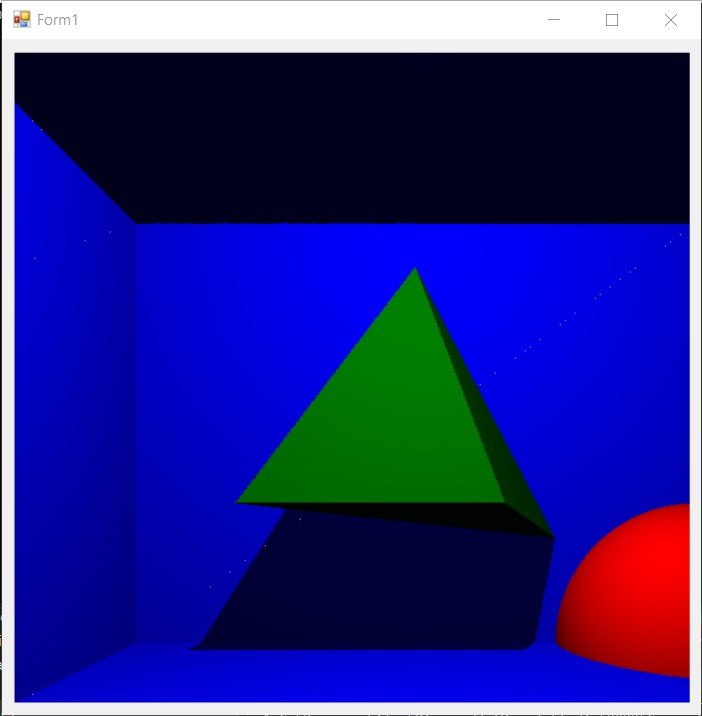
\includegraphics[width=1\linewidth]{inc/img/demographics}
	\caption{Полученное изображение в результате работы алгоритма}
	\label{fig:test}
\end{figure}

\section*{Вывод}

Были реализованы алгоритмы, а именно алгоритм линии конвейера и последовательный алгоритм обратной трассировки лучей.
